

\newcommand{\VMDIFF}[0]{{\textDelta VM}}
\newcommand{\PROCDIFF}[0]{{\textDelta Proc}}


\begin{table*}
\centering
\begin{tabular}{lrrrr|rrr}
\toprule
\textbf{Benchmark} & \textbf{Instr} & \textbf{LocalVars} & \textbf{\PROCDIFF} & \textbf{\VMDIFF} & \textbf{LocalVars/Instr} & \textbf{\PROCDIFF/Instr} & \textbf{\VMDIFF/Instr} \\
\midrule
\texttt{noploop} & 72.00 & 75.00         & \textbf{13.63} & 17965.51
                         & 1.04$\times$  & 0.19$\times$   & 249.52$\times$ \\
\texttt{pivoter} &\textbf{226.12} & 260.52       & 516.30        & 23399.51
                                  & 1.15$\times$ & 2.28$\times$  & 103.48$\times$ \\
\texttt{kmeans} & \textbf{270.00} & 9136.11       & 51417.96       & 254554.27
                                  & 33.84$\times$ & 190.44$\times$ & 942.79$\times$  \\
\texttt{omp} & \textbf{3593.00} & 457358.41      & 832265.90      & 130034289.69 
                                & 127.29$\times$ & 231.64$\times$ &	36191.01$\times$  \\
\bottomrule
\end{tabular}
\caption{Average checkpoint sizes (in bytes) across filtered iterations. "Instr" refers to the instrumented version produced by our static analysis-based checkpointing. "\PROCDIFF" and "\VMDIFF" refer to memory diffs at the process and virtual machine levels respectively.}
\label{tab:checkpoint-sizes}
\end{table*}

\begin{figure*}
    \centering
    % \tikzset{external/force remake}

% \PlotExp{<Title>}{<CSV path>}{<Prefix>}
\newcommand{\PlotExp}[3]{%
  % \DependOnCSV{#2}% ensures rebuild if the CSV changes
  \nextgroupplot[title={#1}]
  \pgfplotstableread[col sep=comma,trim cells]{#2}\datatable

  % Per-row bands for proc0..4
  \pgfplotstablecreatecol[
    create col/expr={min(min(min(min(\thisrow{proc0},\thisrow{proc1}),\thisrow{proc2}),\thisrow{proc3}),\thisrow{proc4})}
  ]{procmin}{\datatable}
  \pgfplotstablecreatecol[
    create col/expr={max(max(max(max(\thisrow{proc0},\thisrow{proc1}),\thisrow{proc2}),\thisrow{proc3}),\thisrow{proc4})}
  ]{procmax}{\datatable}

  % Per-row bands for vm0..4
  \pgfplotstablecreatecol[
    create col/expr={min(min(min(min(\thisrow{vm0},\thisrow{vm1}),\thisrow{vm2}),\thisrow{vm3}),\thisrow{vm4})}
  ]{vmmin}{\datatable}
  \pgfplotstablecreatecol[
    create col/expr={max(max(max(max(\thisrow{vm0},\thisrow{vm1}),\thisrow{vm2}),\thisrow{vm3}),\thisrow{vm4})}
  ]{vmmax}{\datatable}

  % Bands (unique name paths via prefix #3)
  \addplot[name path=#3PROCmax, draw=none] table[x=i, y=procmax]{\datatable};
  \addplot[name path=#3PROCmin, draw=none] table[x=i, y=procmin]{\datatable};
  \addplot[fill opacity=0.14, draw=none] fill between[of=#3PROCmax and #3PROCmin];

  \addplot[name path=#3VMmax, draw=none] table[x=i, y=vmmax]{\datatable};
  \addplot[name path=#3VMmin, draw=none] table[x=i, y=vmmin]{\datatable};
  \addplot[fill opacity=0.14, draw=none] fill between[of=#3VMmax and #3VMmin];

  % Central lines
  \addplot[very thick] table[x=i, y=procavg]{\datatable};
  \addplot[very thick, dashed] table[x=i, y=vmavg]{\datatable};
  
    \addplot[
      only marks,
      mark=diamond*,
      mark options={blue}
    ] table[x=i, y=naive]{\datatable};
    
    \addplot[
      only marks,
      mark=asterisk,
      mark options={red}
    ] table[x=i, y=instrumented]{\datatable};
}

% \tikzsetnextfilename{benchmarks-fourpanel} % cache file: tikz-cache/benchmarks-fourpanel.pdf
\begin{tikzpicture}
\begin{groupplot}[
    group style={
        group size=2 by 2,
        horizontal sep=2cm,
        vertical sep=2cm
    },
    width=0.48\textwidth,
    height=0.35\textwidth,
    xlabel={iteration},
    ylabel={bytes},
    ymode=log,
    %xtick=\empty,
    xticklabel={\tiny\pgfmathprintnumber{\tick}},
    %xtick distance=1,
    % ymin=9,
    % ymax=3e8,
    grid=major,
    title style={yshift=-1ex},
    legend to name=grouplegend,
    legend columns=4,
    legend style={/tikz/every even column/.append style={column sep=1em}, draw=none, font=\small, anchor=north}
]

\PlotExp{\texttt{noploop}}{experiments/noploop.csv}{A}
\PlotExp{\texttt{pivoter}}{experiments/pivoter.csv}{B}
\PlotExp{\texttt{kmeans}}{experiments/kmeans.csv}{C}
\PlotExp{\texttt{omp}}{experiments/omp.csv}{D}

\end{groupplot}

\end{tikzpicture}
\vspace{1ex} % optional spacing
\begin{center}


%\pgfplotslegendfromname{grouplegend}
% Define legend items here (OUTSIDE the plot):
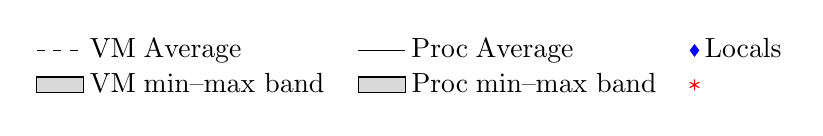
\begin{tikzpicture}
  \begin{axis}[
      hide axis,
      scale only axis,
      xmin=0, xmax=1, ymin=0, ymax=1, % force non-empty range
      legend columns=3,
      legend style={draw=none, /tikz/every even column/.append style={column sep=1em}}
    ]

    \addlegendimage{line legend, black, dashed}
    \addlegendentry{\VMDIFF\;Average\qquad\quad\ }

    \addlegendimage{line legend, black}
    \addlegendentry{\PROCDIFF\;Average\qquad\quad\ }

    \addlegendimage{only marks, mark=diamond*, mark options={blue}}
    \addlegendentry{Locals}
    
    \addlegendimage{area legend, fill=black!15, draw=none}
    \addlegendentry{\VMDIFF\;min--max band}

    \addlegendimage{area legend, fill=gray!30, draw=none}
    \addlegendentry{\PROCDIFF\;min--max band}

    \addlegendimage{only marks, mark=asterisk, mark options={red}}
    \addlegendentry{\spyte}

  \end{axis}
\end{tikzpicture}
%\end{comment}
\end{center}

\end{figure*}

\section{Evaluation}
\label{sec:evaluation}
We evaluate our approach to program-guided checkpointing on four Python workloads: \texttt{noploop}, \texttt{pivoter}, \texttt{kmeans}, and \texttt{omp}. These benchmarks capture common iterative patterns in numerical computing and machine learning, with varying degrees of control complexity, memory reuse, and heap allocation behavior. In each, we insert checkpoint instrumentation at the head of the primary loop, allowing recovery from the beginning of any iteration. We measure the size of the persisted state after each checkpoint operation.

\begin{itemize}
    \item \textbf{noploop} is a degenerate \texttt{range} \texttt{for} loop with no meaningful computation or allocation except the iterator. It serves as a lower bound on checkpointing overhead. We run the loop for 100 steps.

    \item \textbf{pivoter} (26 LOC, 2 out of 7 relevant variables) performs clique enumeration over a sparse graph via depth-first search and backtracking. Program state is encoded in sets and counters. Input is a 100-node, 757-edge subgraph extracted from the Enron dataset. The algorithm requires $\sim 47,000$ steps to complete. Due to the computational cost of process- and VM-level checkpointing, we sample checkpoints every 50 or 51 steps (yielding 1,891 checkpoint pairs total), but measure memory differences between consecutive snapshots to estimate per-step deltas. This avoids the cost of capturing all 47,000 steps while maintaining fair comparison granularity.

    \item \textbf{kmeans} (15 LOC, 1 out of 10 relevant variables) implements K-means clustering on synthetic data. Each iteration reassigns samples to centroids and updates them. Only the centroid array needs to persist. Data is generated using \texttt{sklearn.datasets.make\_blobs} with $n\_samples=1000$, $n\_features=2$, $k=5$. The algorithm completes in 20 steps.

    \item \textbf{omp} (42 LOC, 2 out of 21 relevant variables) --- Orthogonal Matching Pursuit is a greedy feature selection algorithm. At each step, it selects the feature most correlated with the residual and retrains a regression model from scratch. The input is the \texttt{healthstudy} dataset with $k = 35$. The algorithm completes in 35 steps.
\end{itemize}

All benchmarks use fixed data and identical loop structure across checkpointing configurations. Dataset selection was finalized before implementing or evaluating instrumentation.

\begin{itemize}
  \item \textbf{LocalVars}: Pickling all local variables (excluding parameters), regardless of whether they were modified or needed again.
  \item \textbf{\PROCDIFF}: We implemented process-level checkpointing using a custom tool that captures all writable memory regions by reading from \texttt{/proc/self/mem}. We initially attempted to use CRIU for process-level checkpointing, but found its memory overhead dominated the storage costs by orders of magnitude, making meaningful comparison impossible. 
  \item \textbf{\VMDIFF}: VM-level checkpointing based on snapshots and 64-byte memory diffing between iterations. The checkpoints are taken by triggering QEMU memory dumps via QMP commands over TCP.
\end{itemize}

We omit the first iteration of each benchmark (since no diff can be computed). We also omit the final two iterations, which introduce irregularities in the {\PROCDIFF} and {\VMDIFF} baselines.

\paragraph{Notes on Overhead Accounting}
The use of TCP to trigger VM-level checkpoints may introduce a nontrivial fixed overhead per snapshot, including QEMU internals and I/O latency. While the precise size impact of this mechanism is difficult to isolate, we partially control for such effects by comparing deltas between consecutive snapshots rather than absolute snapshot sizes. In contrast, the analysis-based and LocalVars Python checkpoints use direct pickle serialization. Thus, while our VM-level measurements reflect realistic system-level behavior, they may slightly overestimate true memory diffs compared to language-level checkpointing.

\subsection{Checkpoint Size Comparison}

Table~\ref{tab:checkpoint-sizes} reports the mean size in bytes of each checkpointing method after filtering. Our system consistently outperforms both LocalVars Python checkpointing and simulated Process- and VM-level methods.

For the noploop benchmark, our analysis incurs a fixed overhead (iterator) that exceeds 
the minimal state changes, making process-level diffing more efficient. This 
represents a limitation for programs with very small persistent state.

The \texttt{pivoter} benchmark---a recursive clique enumeration kernel --- maintains small internal state (e.g., recursion depth and adjacency buffers) that is genuinely required to resume computation. Our system’s performance is nearly identical to the process-level memory diff, suggesting that it is near-optimal in this case; in contrast, naively checkpointing all local variables leads to 10x memory overhead. The \texttt{noploop} benchmark confirms the lower bound: our instrumentation adds minor overhead (e.g., iterator state), while process-level diffing captures the true minimal footprint. Comparing \texttt{\PROCDIFF} results between \texttt{pivoter} and \texttt{noploop} reveals that process snapshots can be highly efficient in simple cases, adding as little as 23 bytes of overhead.

By contrast, in \texttt{kmeans}, the difference is driven by transient arrays such as gradients, distances, and cluster metrics, all of which are allocated per iteration and dead by the loop's end. The \texttt{omp} benchmark benefits even more dramatically: while it uses large working arrays and regression buffers, these are reused rather than persisted, and are excluded from checkpoints by the dirty-pointer analysis.

These results show that the combination of static analysis and lightweight dynamic instrumentation can exclude large volumes of memory that are either unmodified or recomputable, particularly in numerical programs with regular iterative structure.

\subsection{Discussion}

The results support the following observations:

\begin{itemize}
  \item \textbf{Static analysis can yield substantial reductions} in checkpoint size when recomputation is cheap and allocation is disciplined. This aligns with common usage patterns in numerical and data science code.
  \item \textbf{VM- and Process-level diffs greatly overapproximate state necessity}: they include any mutated memory, even if transient or unused, leading to high checkpoint costs.
  \item \textbf{Analysis precision is workload-sensitive}: the benefits are most pronounced when mutable state is well-localized, heap aliasing is limited, and control structure is predictable.
\end{itemize}

\subsection{Limitations and Threats to Validity}
\label{sec:threats}

Our system assumes that all side effects are either annotated or internal to the function body. If external state is mutated (e.g., global variables, files, sockets) and not captured by the type system, recovery may be unsound.

Additionally, our analysis does not verify behavioral equivalence post-recovery. We produce an explicitly instrumented code so the programmers can double-check it by themselves. we rely on programmer discipline and the assumption that the relevant control path is idempotent from the checkpoint location onward.

Our analysis takes a few seconds per benchmark function, and can be run entirely ahead-of-time. This is fast enough to be usable in practice and supports iterative development. We do not report fine-grained performance numbers, as the tool is not designed to operate online or scale to large codebases; rather, its value lies in enabling precise transformations in tightly scoped, performance-critical numerical kernels.
